% 12 pt, 1 inch margin, 1.5 line spacing
\documentclass[12pt, oneside]{article}
\usepackage{geometry}
\geometry{letterpaper, margin=1in}

\usepackage[utf8]{inputenc}
\usepackage[T1]{fontenc}
\usepackage[english]{babel}
\usepackage{graphicx}
\usepackage{amssymb}
\usepackage{authblk}
\usepackage{setspace}
\usepackage{tabularx}
\onehalfspacing


% changes Twitter to be specific
\title{Measuring and Forecasting Influenza Outbreaks Using Twitter}

\author[1]{Tianyu Chen}
\author[2]{Yuhan Zeng}
\author[1]{Rui Zhang}
\affil[1]{Department of Computer Science, Indiana University}
\affil[2]{Department of Chemistry, Indiana University}
\affil[ ]{\textit{chen512@indiana.edu, \{rz20, yuhzeng\}@iu.edu}}
\renewcommand\Authands{, }
\date{\today}

\begin{document}
\maketitle



\section{Objectives and Significance}

% Briefly introduce the significance of the project. About 2 paragraphs

Infectious diseases are one of the major causes of morbidity and mortality, among which influenza is a ubiquitous epidemic \cite{hickmann2015forecasting}.
Commonly known as ``the flu'', it is caused by influenza virus and can be a highly infectious disease whose symptoms include runny nose, (high) fever,
sore throat, headache, coughing and fatigue\cite{wiki:flu}. Although there are numerous studies about predicting and forecasting the trend of influenza outbreaks,
there are some limitations still, specifically of their source of data. Related studies commonly leverage influenza-like illness (ILI) and severe acute
respiratory infections (SARI) data, which is defined by WHO\cite{world2014global}. Take the \textit{Influenza Observation and Forecast} system that is part of
Columbia Prediction of Infectious Disease (CPID) maintained by Columbia University \cite{cpid} for example, it only tracks the data from a total of 38 out of
195 sovereignties in the world today. Furthermore, its frequency of prediction can be limited by the publication of the corresponding data source.

To mitigate the problems above, we propose an epidemic outbreak prediction technique based on analyzing the data gathered from popular social media
like Twitter. Compared with the traditional approach, a noteworthy advantage of social media information is its ubiquitousness and timeliness
- end users are producing such data wherever and whenever they are. By performing a keyword-based text mining based on an anonymized tweet dataset and utilizing
the geographic information as a supplement, we can forecast whether a influenza outbreak is expected in near future.


\section{Background}

% 1. Introduce all important concepts and background information
% 2. Search the literature and describe previous work on this problem
% 3. If there exists previous work on the problem, describe what makes your work particularly interesting

\subsection{Predicting the Flu}

Influenza, often called ``the flu'', is an acute respiratory illness that infects approximately 10 - 15\% of the people around the world each year.
It can be deadly. For example in 2009, pandemic H1N1 (\textit{``swine flu''}) is estimated to result in 12,469 deaths in the United States \cite{H1N1}.
The early detection of influenza is of paramount importance to timely contain the spread of the illness. In the United States, Centers for Disease Control and Prevention (CDC)
report an influenza-like illness (ILI) index weekly based on the data collected from medical practices in a surveillance network. However, this report process is almost
entirely manual and there is a typical 1 - 2 week delay due to the lag in clinical data acquisition \cite{TwitterSeasonalFlu}.
Given the increasing demand for epidemic monitoring and forecasting in real time, web and social media (such as Google \cite{GoogleFlu} and Twitter \cite{TwitterFlu})
emerge as a new data source \cite{MediaFlu}.

\subsection{Twitter Text Mining}

Twitter, an online micro-blogging (limited to 280 characters) and social network service, has an average of 330 million active users worldwide \cite{TwitterUser} each month.
It could be a promising data source for the early detection of ILI due to its timeliness, public availability, and popularity \cite{TwitterAnalyzeMessage}.
Paul et al. \cite{TwitterWorldWide} shows that influenza-related tweets were positively correlated ($r$: 0.37 - 0.81) with existing government surveillance data
in 10 English-speaking countries.

\subsubsection{APIs}
\label{subsubsec:api}

\begin{table}[h]
  \centering
  \caption{A list of Twitter APIs}
  \label{table:api}
  \begin{tabularx}{.75\textwidth}{ |c|c|X| }
    \hline
    \textbf{Parameter} & \textbf{Required} & \textbf{Function} \\
    \hline
    \hline
    q & Yes & The query string, 500 chars max \\
    \hline
    geocode & No & Specifying the latitude/longitude as well as the radius \\
    \hline
    lang & No & ISO 639-1 language code, restricting the results \\
    \hline
    locale & No & Specifying the language of the query string \\
    \hline
    result\_type & No & Has 3 values: \textit{recent} (only recent results), \textit{popular} (only popular ones) and \textit{mixed} (all tweets) \\
    \hline
    count & No & The number of tweets returned \\
    \hline
    until & No & Tweets created before a specific date \\
    \hline
  \end{tabularx}
\end{table}


% Briefly introduce a few useful APIs provided by Twitter
The Twitter API is an interface that takes a query as input and returns a JSON containing relative tweets and metadata as output.
In Table ~\ref{table:api} some parameters that we are interested in are listed with their functionalities.

\subsubsection{Related Research}

A variety of data mining and machine learning techniques have been applied to Twitter data analysis and influenza trend prediction.
Santillana et al. \cite{Santillana} combine multiple ILI activity estimates into a single prediction of ILI using machine learning ensemble approaches,
which produces accurate weekly ILI predictions for up to four weeks ahead of CDC's ILI reports. Santos et al. \cite{Santos} show that by changing data pre-processing and
feature extraction and selection the Naive-Bayes classifier and regression model built to predict the flu can be adapted to languages other than English.
Aron Culotta \cite{Culotta} proposes a document classifier to filter the \textit{misleading} messages, which significantly reduce error rate in simulated false alarm experiments.
Li et al. \cite{Li} build up a real-time ILI reporting system based on Flu Markov Network (Flu-MN), an unsupervised Bayesian algorithm based on a 4 phase Markov Network.
Chen et al. \cite{Chen} propose both an unsupervised model and an improved supervised weakly model that captures the hidden states of a user from her tweets
and estimates the flu trend. Aramaki et al. \cite{Aramaki} describe a support vector machine (SVM) based classifier that shows high correlation (0.97)
at the outbreak and early spread. Achrekar et al. \cite{TwitterSeasonalFlu} show that text mining significantly enhances the correlation between the Twitter and CDC reported ILI rates.

In particular, Lee et al. \cite{TwitterSurveillance} reports a real-time flu surveillance system leveraging data mining on tweets. However, their approach only accounts for
a few most \textit{frequent} words that co-occurs with a disease name, which seems na\"{i}ve in that the model overlooks \textit{infrequent} keywords related to flu outbreak.
They update their system in 2017 \cite{TwitterNNs} using multilayer perceptron. Compared to their previous work, it shows an improved accuracy.
However, only promoting tweets (ads) and the repeated ones are filtered.

\section{Proposed Approach}

\subsection{Data Collection}
\label{subsec:data_collection}

% 1. Describe your data and how you will obtain it
Social media like Twitter and Facebook plays an important role in our daily life today. Organizations such as Centers for Disease Control and Prevention
(CDC) collect weekly influenza test results from public health laboratories and make infection prediction with an inevitable delay of up to two weeks.
For a more timely and efficient prediction of influenza, we collect a vast number of tweets that fall into a particular time span and extract related data
from them. Owing to the popularity and timeliness of Twitter posts, they can be used to assess health status or predict the spread and fluctuation of an epidemic
in a certain population in real-time.

To retrieve the dataset, we plan to use the Twitter APIs (introduced in ~\ref{subsubsec:api}) to collect text tweets during a certain time span and in a particular
geographic space. A few keywords such as ``flu'', ``influenza'' and ``H1N1'' will be used to restrict the content of tweets to be collected.
However, since not all tweets collected with the keywords can be considered as an indication of real-time illness, the raw data needs to be filtered to further
remove irrelevant entries. We plan to train a bag-of-words (BOW) classifier using regression to predict whether a Twitter post containing certain keywords of interest
indicates that the Twitter user shows signs of influenza infection. In addition, redundant information such as re-tweets, duplicate tweets (in terms of content)
and tweets by a same user within a time threshold will be cleaned from the dataset.


\subsection{Methodology}

% 2. Describe your proposed method and implementation in detail

\subsubsection{Keyword Extraction}
To provide a better insight of a Twitter-based influenza trend forecast, we propose to extract the keywords by performing text mining on the dataset collected
using the methodology described in ~\ref{subsec:data_collection}. We propose a random forest (RF) based word sampling method to calculate the significance of a keyword.

\paragraph{Random Forest}
A random forest is an ensemble of decision trees grown from the bootstrap dataset - the bootstrap means independently and uniformly sampling a subset of data with replacement.
In each decision tree, the attribute is the presence of selected word (either 0 or 1) and the output is the influenza trend (i.e. \%-weighted ILI).

The Gini index is used to split a node:

$$GINI_{split} = \sum_{i=1}^{k}\frac{n_i}{n}GINI(i)$$ 

The Gini score computed over all decision trees will then be used to rank the word.

\paragraph{Word Sampling}
In this step, the Wilcoxon rank-sum test \cite{WilcoxonRankSum} will be used to compare the Gini score of a word with that of a random generated ``noise word'' to determine
the significance of the word of interest. The null hypothesis ($H_0$) is the mean Gini score of a given word is the same as that of the random ``noise word''.
As for the ``noise word'', a number of words will be picked randomly from a dictionary and selected only when it has no \textit{prediction power}.
A significance threshold $\theta$ will be chosen to remove all the trivial words (i.e. the words whose p-value is greater than $\theta$).
Additionally, we plan to evaluate the correlation between the words and the influenza trend using $\chi^2$-test, which could assist keyword selection in case
the sampling method described above fails.


\subsubsection{Predictive Model}

The proposed predictive model is based on the one descibed in K. Lee et al., 2017 \cite{lee2017forecasting}. As a supplement, we plan to combine the ILI-related physician visit
percentage with keyword frequencies appeared in different tweets as in the original paper. The influenza statistic after a week is produced as output.
A major improvement over the original approach is that by introducing a filter before the layered perceptron, those apparently irrelevant tweets can be filtered
in advance using heuristics. This can improve the efficiency of the perceptron especially when the number of the tweets on which our forecast is based is relatively large.

\subsection{Evaluation}
\label{subsec:evaluation}

% 3. Describe evaluation strategy in detail
We propose 3 evaluation metrics to measure the performance of our method. These measures will be employed in text mining and also in the predictive model part if applicable.

\paragraph{Pearson Correlation}
Pearson Correlation ($r$) is a measure of the linear correlation between two variables $X$ and $Y$ \cite{wiki:correlation}.

$$ r = \frac{\sum_{i=1}^n(x_i-\bar{x})(y_i-\bar{y})}{\sqrt{\sum_{i=1}^n(x_i-\bar{x})^2}\sqrt{\sum_{i=1}^n((y_i-\bar{y})^2}}$$

\paragraph{Root Mean Squared Deviation}
Root Mean Squared Deviation (RMSD) is a measure of the difference between predicted and real values \cite{wiki:root-mean-square}.

$$RMSD = \sqrt{\frac{\sum_{i=1}^{n}(\hat{y}-y_i)^2}{n}}$$

In keyword extraction, it can be benefitial to observe the RMSD of keywords over a certain period of time $t$.

\paragraph{Precision}
Precision is a fraction where the number of the documents relevant to the user's information is divided by the total number of documents. By definition we have:

$$PPV = \frac{TP}{TP+FP}$$


\subsection{Expected Outcome}

% 4. Describe expected outcomes with a fall back on option in case the initial idea fails

\begin{figure}[h]
    \centering
    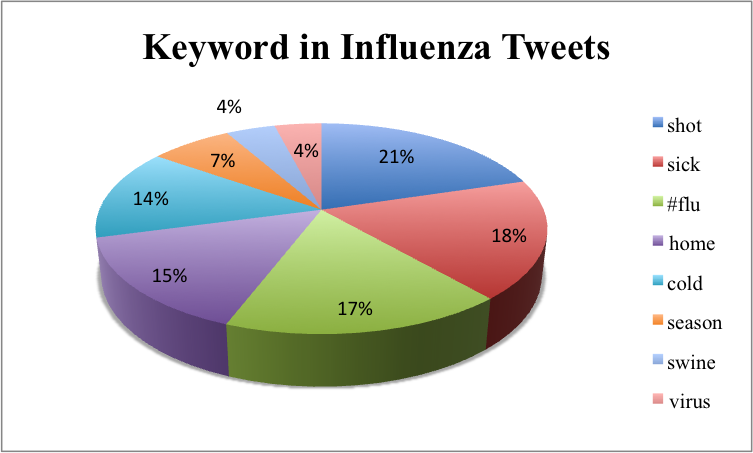
\includegraphics[width=0.7\textwidth]{TweetsWords.png}
    \caption{The example of expected outcome for keywords extraction}
    \label{fig:fig1}
\end{figure}

\begin{figure}[h]
    \centering
    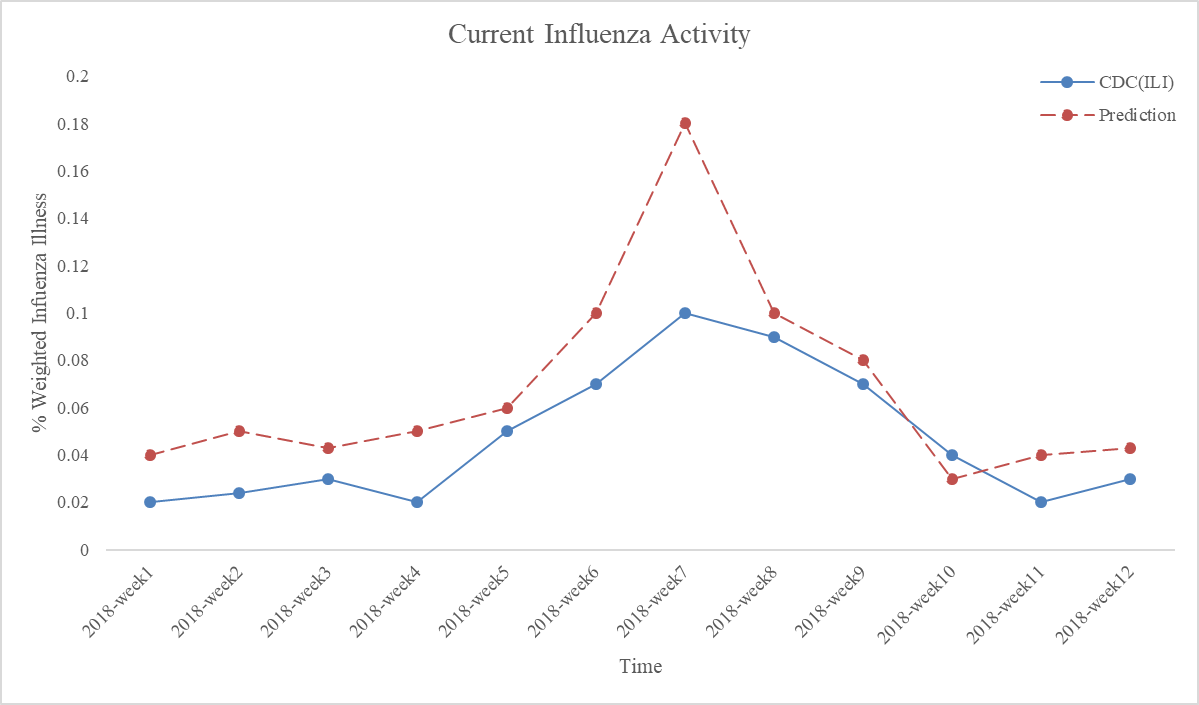
\includegraphics[width=0.7\textwidth]{predictions.png}
    \caption{The example of expected outcome for Predictive Model}
    \label{fig:fig2}
\end{figure}

We expect to extract a list of keywords from the tweets with a high correlation with the actual flu trend. In terms of the visualization, we will plot the
frequency of keywords (similar to the one shown in Figure ~\ref{fig:fig1}). As a backup option, we may perform text mining using Twitter Latent Dirichlet
Allocation (LDA) model for trend prediction, where there are many open-source libraries available for implementation. However the issue with the LDA model is that
the words generated may not signal an actual flu outbreak.

We expect to predict the flu trend 1 - 2 weeks ahead of the release of CDC reports. To visualize the prediction, we will plot our predictive model in the
current flu activity (i.e., percentage of ILI-related physicians visit) in weekly time-series (similar to the one shown in Figure ~\ref{fig:fig2}.
As a fallback option, we could use support vector machine (SVM) classifier as reported by Aramaki et. al \cite{Aramaki}. However, SVM tends to
overfit the flu trend and may need a longer training time due to the size of the Twitter dataset.


\section{Individual Tasks}

% Describe what each member of the team will do

\begin{table}[h]
  \centering
  \begin{tabularx}{0.8\textwidth}{ |c|X| }
    \hline
    \textbf{Member} & \textbf{Task Summary} \\
    \hline
    \hline
    Rui Zhang & Develop and perform experiments   \\
    \hline
    Yuhan Zeng & Develop and perform experiments  \\
    \hline
    Tianyu Chen & Process and analyze data, doing documentation  \\
    \hline
  \end{tabularx}
  \caption{Task allocations}
  \label{table:role}

\end{table}

\paragraph{Rui Zhang}
Rui Zhang is responsible for system development as well as performing experiments to collect data and analyze the result.

\paragraph{Yuhan Zeng}
Yuhan Zeng, leveraging her data science skills, is responsible for data processing and analysis. She is also responsible for the storage and access of the Twitter dataset.
She will also ensure the correctness of the implementation by testing.

\paragraph{Tianyu Chen}
Tianyu Chen will lead the code development. He is also responsible for testing and assisting other team members.

Depending on the actual project progress, additional task or work may be assigned to each team member.

\section{Expected Outcome}

We expect that our predictive model can generate a similar influenza outbreak trend with the CDC report, measured by the 3 evaluation approaches
mentioned in ~\ref{subsec:evaluation}.


\bibliographystyle{unsrt}
\bibliography{ref}

\end{document}
